\section{I-Measure}


\subsection{Definition}
\begin{frame}{Definition}
    \begin{definition}[Field]
        The field $\mathcal{F}_{n}$ generated by sets $\tilde{X}_{1}, \tilde{X}_{2}, \cdots, \tilde{X}_{n}$ is the collection of sets which can be obtained by any sequence of usual set operations (union, intersection, complement, and difference) on $\tilde{X}_{1}, \tilde{X}_{2}, \cdots, \tilde{X}_{n}$
    \end{definition}
    
    
    \begin{definition}[Atom]\label{atom}
    The atoms of $\mathcal{F}_{n}$ are sets of the form $\cap_{i=1}^{n} Y_{i},$ where $Y_{i}$ is either$\tilde{X}_{i}$ or $\tilde{X}_{i}^{c},$ the complement of $\tilde{X}_{i}$\\
    \end{definition}
    
    
    \begin{definition}[Signed Measure]\label{sm}
    A real function $\mu$ defined on $\mathcal{F}_{n}$ is called a signed measure if it is set-additive, i.e., for disjoint $A$ and $B$ in $\mathcal{F}_{n}$
    \begin{equation}
    \mu(A \cup B)=\mu(A)+\mu(B)
    \end{equation}
    \end{definition}

\end{frame}


\subsection{Measure Theorem}
\begin{frame}{Measure Theorem}
    
    Use $X_{G}$ to denote $\left(X_{i}, i \in G\right)$ and $\tilde{X}_{G}$ to denote $\cup_{i \in G} \tilde{X}_{i}$ for any nonempty subset $G$ of $\mathcal{N}_{n} =\{1,2, \cdots, n\}$\\
 

    \begin{theorem}[Completeness]\label{th1}
    Let
    \begin{equation}
        \mathcal{B}=\left\{\tilde{X}_{G}: G \text { is a nonempty subset of } \mathcal{N}_{n}\right\}
    \end{equation}
    Then a signed measure $\mu$ on $\mathcal{F}_{n}$ is completely specified by $\{\mu(B), B \in \mathcal{B}\}$
    which can be any set of real numbers.
    \end{theorem}
    
    With the terminologies of measure theory above, we can construct a correspondence between set theory and Shannon Information
    
    
\end{frame}

\subsection{Correspondence}

\begin{frame}{Correspondence}
    \begin{block}{Build Correspondence}
    We now construct the I-Measure $\mu^{*}$ on $\mathcal{F}_{n}$ using Theorem \ref{th1} by defining%%%%%%%%%%%%%
    \begin{equation}
        \mu^{*}\left(\tilde{X}_{G}\right)=H\left(X_{G}\right)
    \end{equation}
    for all nonempty subsets $G$ of $\mathcal{N}_{n} .$ 
    
    The following must hold for all (not necessarily disjoint) subsets $G, G^{\prime}, G^{\prime \prime}$ of $\mathcal{N}_{n}$:
    \begin{equation}\label{eqx1}
        \mu^{*}\left(\tilde{X}_{G} \cap \tilde{X}_{G^{\prime}}-\tilde{X}_{G^{\prime \prime}}\right)=I\left(X_{G} ; X_{G^{\prime}} | X_{G^{\prime \prime}}\right)
    \end{equation}
    \end{block}
\end{frame}


\subsection{Applications}
\begin{frame}{Applications}
    \begin{block}{Information Diagrams}
        With the correspondence above, it is reasonable to use an \emph{information diagram}, which is a variation of Venn diagram, to represent the relationship between Shannon's information measures.
    \end{block}
    \begin{figure}
        \centering
        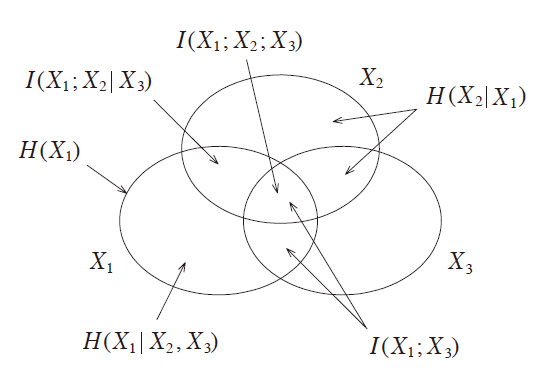
\includegraphics[height = 3cm]{img/Im3.png}
        \caption{Generic Information Diagram for $X_1, X_2, X_3$}
        \label{fig:genericID}
    \end{figure}
\end{frame}

\begin{frame}{Applications}
    \begin{block}{Information Diagrams for Zero Measure}
        In Markov Chain $X_{1} \rightarrow X_{2} \rightarrow X_{3}$, since \begin{equation}\mu^{*}\left(\tilde{X}_{1} \cap \tilde{X}_{2}^{c} \cap \tilde{X}_{3}\right)=I\left(X_{1} ; X_{3} | X_{2}\right)=0\end{equation}
        We don't have to plot that region out in the information diagram, making the diagram simpler and more useful when reasoning about Shannon information measures.
    \end{block}
    \begin{figure}
        \centering
        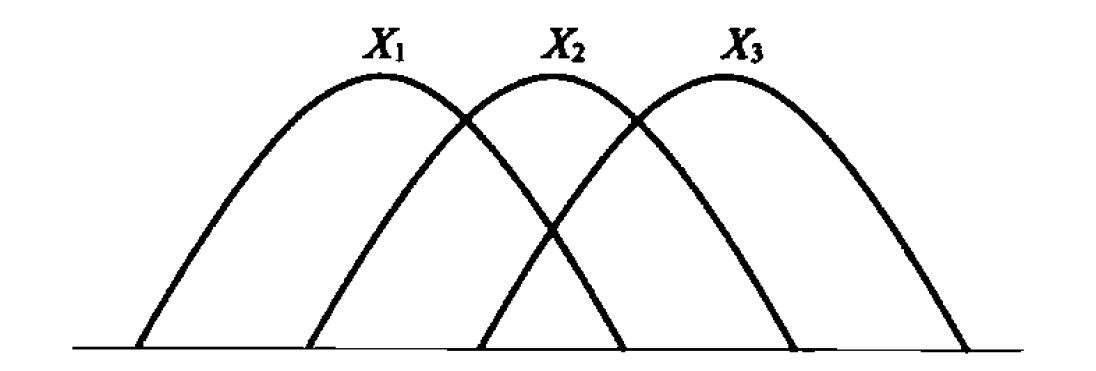
\includegraphics[height = 2cm]{img/Im4.png}
        \label{fig:MCID}
    \end{figure}
    
    In a word, with the set-theoretic view of information diagram, we can discover many useful properties.
\end{frame}
